\chapter{Introduction}\label{ch:1}

\epigraph{Any fool can write code that a computer can understand. Good
programmers write code that humans can understand}{Martin Fowler}

\section{Motivation}

        One of the goals of any software developer is to write quality code. Code that respects company policy, that has a
large test coverage percentange, that uses well defined mechanism thus making it portable on different operating system \ldots{} etc. 
In order to establish the quality of encode and enforce different standards analysis tools where build. Some of the most 
used tools are:
        \begin{description}[labelindent=2cm]
        \item[NullTerminator] It represents a pseudo-automatic refactoring tool which 
        eliminates the null checks by use of the \textbf{Null Object Design Pattern} \cite{tools:nullTerminator}
        \item[Wala Tool]  Developed by IBM Research it implements a series of dataflow
        and type analysis algorithms.
        \item[FindBugs]   Widely used tool to detect common programming language hacks. E.g: A very common mistake is to use \code{LinkedList} instead
of arrays. LinksedList is implemented, as the name suggest, using a simple linked list which has a high complexy, i.e O(n), for accessing elements. Which may not
be what developers usually expect, or know. Another example is \textbf{never compare two urls using URL.equals}. This is because URL.equals resolves the ip of the
website and then compares them, this doesn't work with virtual hosting (try any random url on the net). If you want to look for antipatterns, just look at URL equals
and hashcode they are always inconsistent, slow and usually don't work.
        \item[Intellij IDE] A platform developed by JetBrains which implements over 100 code inspector tools. One example is finding dead code, i.e code that cannot 
be reached during runtime.
        \item[CodePro]   A platform which implements software metrics developed by
        LOOSE Research Group. Goes by the name of INCODE, also \cite{tools:inCode}
        \end{description}

        Most analysis tools share a generic back-end which can be seen in \ref{fig:analysisArchitecture}. The back-end is responseble
for parsing the code in the desired projects and extracting a low-level abstractions / artefacts of the code (e.g the AST of the code). The extracted low-level artefacts,
though usefull, are too granular for most analysis tools, it needs to be processed furthere, resulting in high-level abstractions / artefacts called a \textbf{model}.  This
model is structured according to a \textbf{meta-model} defined and implemented by the developers of the tool \cite{paper:xcore}.

        \begin{figure}
        \centering
        \scalebox{0.5}{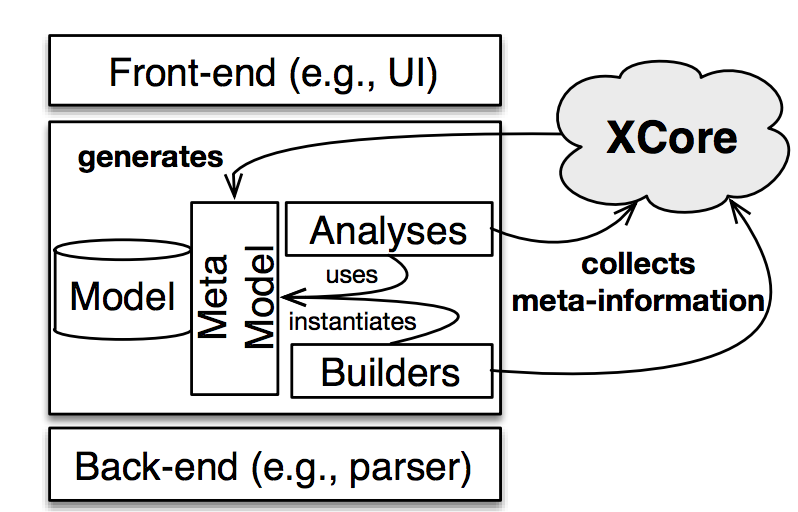
\includegraphics{../img/introduction/analysisArchitecture.png}}
        \caption{Generic Backend for analysis tools \cite{paper:xcore}}
        \label{fig:analysisArchitecture}
        \end{figure}

        The construction of the \textbf{meta-model} is a recuring task when it comes to building analysis tools. \textbf{IPlasma} \cite{tools:iPlasma} uses the \textbf{Memoria}
meta-model in order to compute metrics. Wala \cite{tools:wala} builds its own meta-model in order to preform analysis. Eclipse, as Wala, provides its own meta-model called JDT
\cite{tools:JDT} which is used by most of the Eclipse analysis plugins. 
        
        Building such a meta-model and the necessary back-end is a tedious task, at best. Another major problem that arises when building such a meta-model, and any other program
for that matter, is the evolution in time. We want a meta-mode that can be easily extensible over time, but also have the ability to integrate / inter-operate with other tools / meta-models
in order to obtain complex tools. All of these requirements are difficult to design and implement and, different approaches have been made \cite{tools:fame} \cite{paper:xcore}.

        In order to obtain the mentioned goals, some tools such as inCode\cite{tools:inCode}, have introduced architectural faults which compromised the type safety of the program. This
ultimately lead to poor code which is hard to maintain and understand \cite{oldThesis}.

\section{Previous Work}

        Previously we have build an Ecliplse plugin, called XCore which solved the previously mentioned problems \cite{oldThesis}. The tool works by providing the software developers with
the means to describe the meta-model of their analysis tool directly into the source code of the tool, without the need to actually implement the meta-model. This is done by providing a higher
level of abstraction called meta-meta-model. The meta-meta-model is implemented by using the java annotations system \cite{oldThesis} \cite{book:ThinkingInJava}.

        When the tool is compiled, the java compiler will notice the annotations and invoke the XCore annotation process before actually processing the entire project. Our annotation process
will generate, based on the information provided, the appropriate meta-model for the tool and will enforce all the necessary restrictions on meta-model entities. This is perfectly type safe
because after the code generation phase is over the java compiler can fully typecheck the entire system !
        
\section{Improvements}
        
        XCore provides  a way to describe the necessary meta-model for the analysis tool. It also provides a way to integrated a back-end for the extraction of the "meta-model" from the code.
(e.g it can integrate with the eclipse Jdt for Java meta-mode or Eclipse Cdt for C++ meta-model). In the previous version you could integrate with only one such back-end, but now we have
modified the implementation such that you can integrate with multiple back-ends. 

        Another major feature that we implemented is that one can extend another analysis tool implemented using XCore in order to reuse the functionality from the base tool in the sub-tool.
        Also, we have extended the meta-meta-model description with the concept of Action. One can now describe actions that can be executed upon meta-model entitites. This integrates nicely
with the UI frontend where we could describe an action for opening the analyzed class / method entity in the editor, or concretly pinpoint the design / implementation error from the project
under analysis.

\section{Organization}

        Chapter 2.  Gives a presentation of the XCore tools. We present all the mechanisms that are used by XCore in order to provide the necessary elements for the development of analysis
tools.

        Chapter 3. Gives a thorough presentations of all of XCore's feature. We present this by implementing an analysis tools with three metrics. 

        Chapter 4. In this chapter we summarize all the information
described in previous chapters and present the conclusions. Also, I present the future work which will be done in the development
process of the tool

	 This thesis is an extented refined version of of the paper "XCore: Support for Developing Program Analysis Tools" \cite{paper:xcore}


